\chapter{Teoretický základ}
\section{Sférická soustava souřadnic}
Bod na obloze budeme určovat ve sférické soustavě souřadnic.
Ta umožňuje bod na obloze jednoznačně určit jeho azimutem $\phi$ a zenitem $\theta$.

\begin{definice}[Azimut]\label{def01:1}
  Azimut $\phi$ je úhel na vodorovné rovině, který je svírán se severním směrem. Hodnoty azimutu $\phi$ se pohybují v rozmezí $0^\circ$ až $360^\circ$.
\end{definice}

\begin{definice}[Zenit]\label{def01:2}
  Zenit $\theta$ je úhel vertikálního směru, měřený od bodu přímo nad kamerou (zenit) směrem dolů k horizontu. Hodnoty zenitu $\theta$ se pohybují v rozmezí $0^\circ$ až $90^\circ$.
\end{definice}

Orientaci kamery v terénu pak definujeme pomocí úhlů ($\theta_c, \phi_c$) určujících bod na obloze, který je uprostřed snímku.

\begin{figure}[h]\centering
  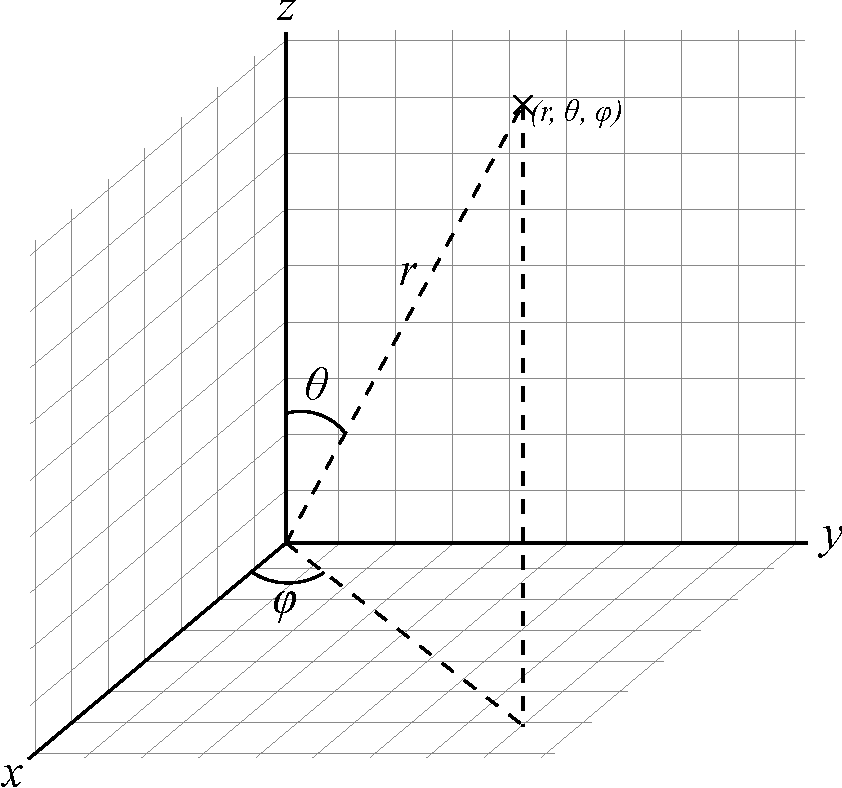
\includegraphics[width=130mm]{../img/spherical}
  \caption{Sférická soustava souřadnic \cite{wiki:spherical}}
\end{figure}


\section{Parametry kamery}

Rozlišujeme vnější a vnitřní parametry kamery.


\subsection{Vnitřní parametry kamery}
Vnitřní parametry kamery jsou např. ohnisková vzdálenost $f_c$, vertikální a horizontální zorný úhel, veliost clony, rychlost závěrky nebo světelnost objektivu.
Nejvýznamější vnitřní parametr objektivu je ohnisková vzdálenost $f_c$, pomocí které lze určit zorné pole kamery.

\begin{definice}[Ohnisková vzdálenost]\label{def01:3}
  Ohnisková vzdálenost $f_c~\text{[mm]}$ je vzdálenost mezi optickým středem objektivu a rovinou snímače (čipu) při zaostření na nekonečno. \citep{Hosko14}
\end{definice}

Ohnisková vzdálenost se mění, když upravujeme optický zoom. Větší zoom znamená větší ohniskovou vzdálenost a užší zorný úhel. 
My budeme ohniskovou vzdálenost modelovat v pixelech, protože neznáme velikost senzoru webových kamer, ale známe rozlišení jejich snímků.

\begin{lemma}\label{lemma01:1}
  Pro objektiv s ohniskovou vzdáleností $f_c~\text{[px]}$ a snímací čip velilosti $(W, H)~\text{[px]}$ je zorný úhel ve vodorovném směru $\omega_h$ dán vztahem
  \begin{equation}\label{eq01:1}
    \omega_h = 2 \arctan \left(\frac{W}{2f}\right).
  \end{equation}
\end{lemma}
\begin{dukaz}
  Vztah je dán goniometrií pravoúhlého trojúhelníku, jehož odvěsny jsou $f$ a $W/2$.
\end{dukaz}

\begin{figure}[h]\centering
  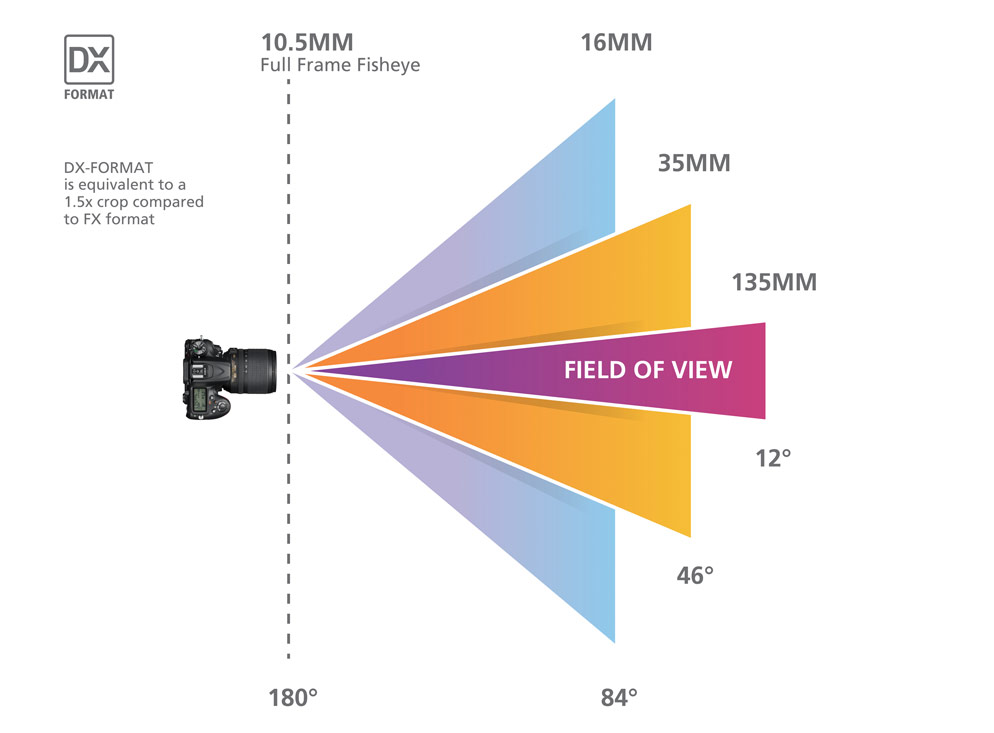
\includegraphics[width=140mm]{../img/fov}
  \caption{Vliv ohniskové vzdálenosti na zorný úhel \cite{nikon}}
\end{figure}

\subsection{Vnější parametry kamery}

Mezi vnější parametry kamery patří její orientace (zenit $\theta_c$, azimut $\phi_c$).
Alternativou, jak popsat směřování kamery, je s pomocí úhlů kolem osy $x$, $y$ a $z$:

\begin{itemize}
    \item $\theta'$ - úhel kolem osy $x$, označovaný jako podélný sklon nebo anglicky pitch, $\theta' = \pi/2 - \theta_c$
    \item $\psi'$ - úhel kolem osy $y$, označovaný jako příčný náklon nebo anglicky roll
    \item $\phi'$ - úhel kolem osy $z$, označovaný jako azimut, kurs nebo anglicky yaw
\end{itemize}



\begin{figure}[h]\centering
    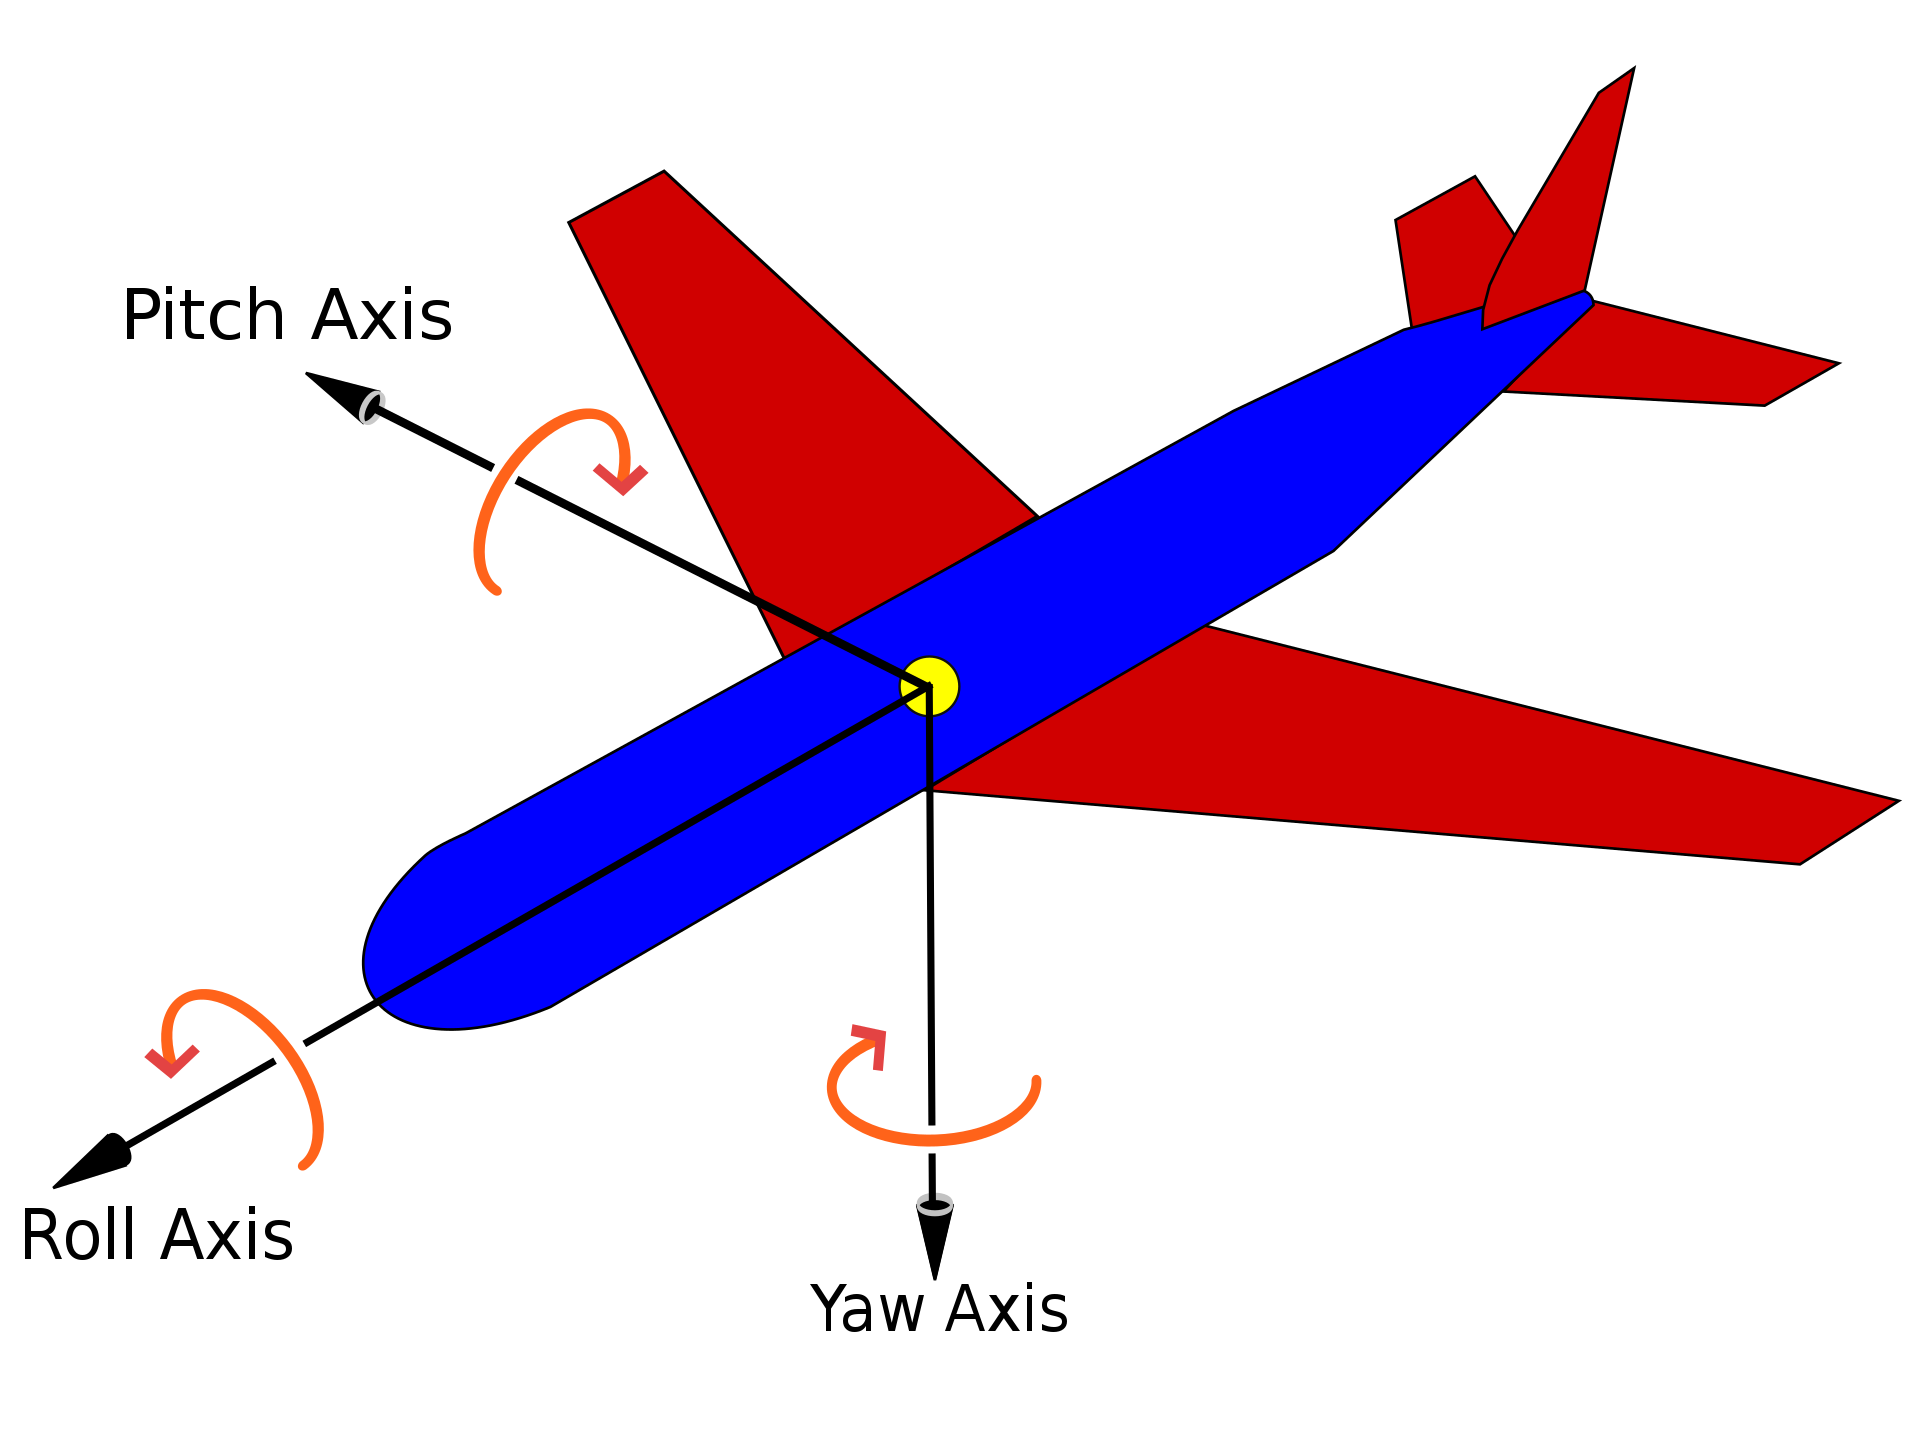
\includegraphics[width=80mm]{../img/rollpitchyaw}
    \caption{Polohové úhly \cite{rpy}}

\end{figure}

\begin{figure}[h]\centering
    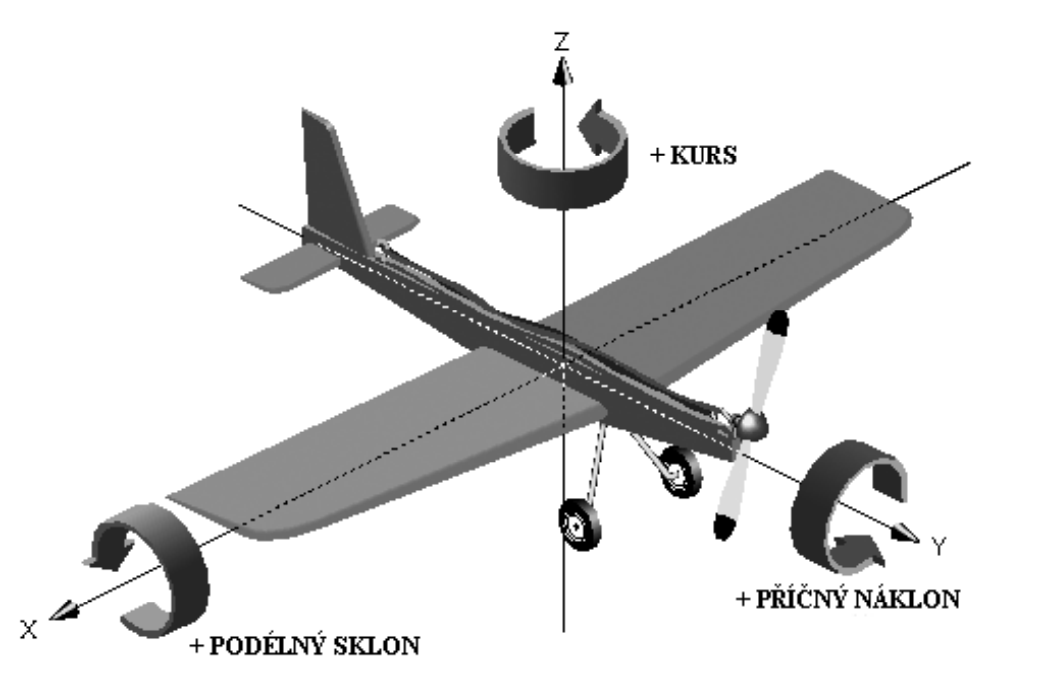
\includegraphics[width=80mm]{../img/naklon}
    \caption{Polohové úhly \citep{Famfulik08}}

\end{figure}

\section{Nalezení bodu na obloze}
Abychom mohli modelovat snímek oblohy kamerou s parametry $(f_c, \theta_c, \phi_c)$, musíme převést pozici pixelu na snímku na pozici bodu na obloze.

\begin{lemma}\label{lemma01:2}(\citealp{Lalonde10}, Appendix B)
  Buď  $\phi_c$ azimut kamery, $\theta_c$ zenit kamery, $f_c~\text{[px]}$ ohnisková vzdálenost kamery, $(W, H)~\text{[px]}$ rozlišení snímku, ($x_p, y_p$) pozice pixelu (horizontální a vertikální vzdálenost od levého horního rohu snímku). Nechť $u_p = x_p - W/2$, $v_p = H/2 - y_p$. Pak
  \begin{equation}\label{eq01:2}
    \theta_p=\arccos \left( \frac{v_p \cdot \sin(\theta_c) + f_c \cdot \cos(\theta_c)}{\sqrt{f_c^2 + u_p^2 + v_p^2}} \right),
  \end{equation}
  \begin{equation}\label{eq01:3}
    \phi_p=\arctan \left( \frac{f_c \cdot \sin(\phi_c) \cdot \sin(\theta_c) - u_p \cdot \cos(\theta_c) - v_p \cdot \sin(\theta_c) \cdot \cos(\phi_c)}{f_c \cdot \cos(\theta_c) \cdot \sin(\phi_c) + u_p \cdot \sin(\theta_c) - v_p \cdot \cos(\theta_c) \cdot \cos(\phi_c)} \right)
  \end{equation}
\end{lemma}
\begin{dukaz}
  Jednotlivé kroky důkazu jsou podrobně popsány v~práci \citet[Appendix B]{Lalonde10}.
\end{dukaz}
  
\begin{lemma}\label{lemma01:3}(\citealp{Lalonde10}, strana 16)
  Nechť $(\phi_c, \theta_c$) je směr kamery, $(\phi_s, \theta_s$) je pozice slunce na obloze, $f_c[px]$ ohnisková vzdálenost kamery, $(W, H)$ rozlišení snímku, ($x_p, y_p$) pozice pixelu (horizontální a vertikální vzdálenost od levého horního rohu snímku). Nechť $u_p = x_p - W/2$, $v_p = H/2 - y_p$. Pak úhel $\gamma_p$ mezi sluncem $(\phi_s, \theta_s$) a bodem na obloze $(\phi_c, \theta_c$) je dán vztahem
  \begin{equation}\label{eq01:4}
    \gamma_p = \arccos \left( \cos(\phi_p) \cdot \cos(\phi_s) + \sin(\phi_p) \cdot \sin(\phi_s) \cdot \cos(\theta_p - \theta_s) \right)
  \end{equation}
\end{lemma}

\begin{figure}[h]\centering
  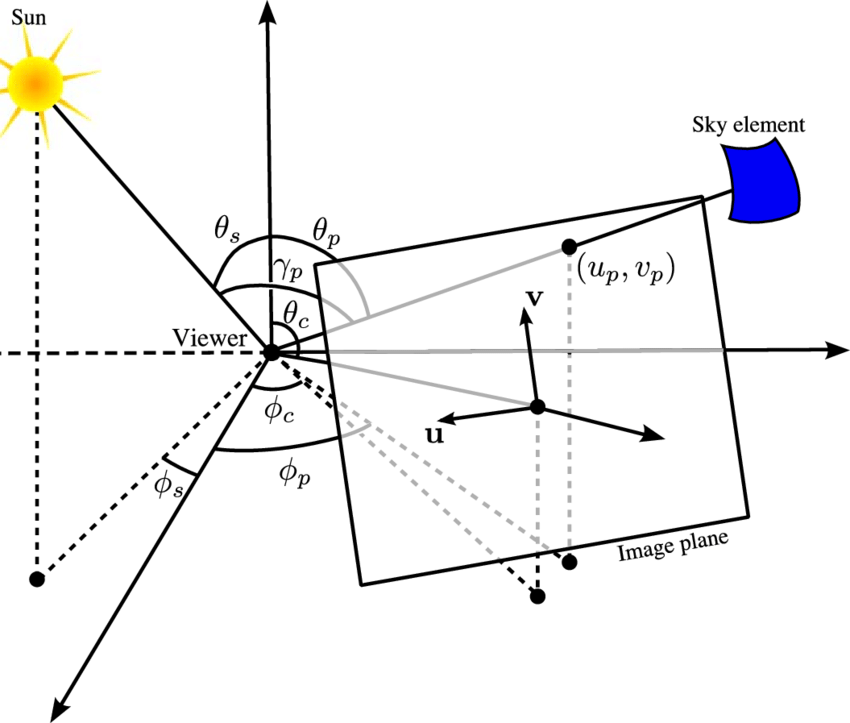
\includegraphics[width=140mm]{../img/uhly}
  \caption{Pozice slunce $(\theta_s, \gamma_s)$, orientace kamery $(\theta_c, \gamma_c)$, pozice bodu na obloze $(\theta_p, \gamma_p)$, úhel bodu na obloze se sluncem $\gamma_p$, pozice bodu na obrázku $(u_p, v_p)$
  (\citealp{Lalonde10}, strana 15)}
\end{figure}

\section{Radiometrie, fotometrie a spektrometrie}
Radiometrie a fotometrie a spektrometrie jsou vědní disciplíny, které se zabývají měřením a analýzou světla a elektromagnetického záření. 
Radiometrie se zaměřuje na kvantitativní měření energie elektromagnetického záření.
Fotometrie se na druhou stranu zaměřuje na měření světla ve vztahu k lidskému vnímání.
Spektrometrie zkoumá vlastnosti světla a elektromagnetického záření v různých vlnových délkách.
Vzhledem k tomu, že lidské oko má různou citlivost na různé vlnové délky světla, fotometrická měření jsou váženy podle vnímání lidského oka. 

Nás nejvíce bude zajímat vztah mezi radiometrickou veličinou zář a fotometrickou veličinou jas.


\begin{definice}[Spektrální odezva]
  Spektrální odezva $V(\lambda)$ je funkce, která popisuje citlivost lidského oka na různé vlnové délky světla.
\end{definice}

\begin{definice}[Spektrální zář a jas]
  Jas $L$ je zář $L_e$ vážená spektrální odezvou lidského oka $V(\lambda)$. Platí:
  \begin{equation}
    L(\lambda) = L_e(\lambda) \cdot V(\lambda)
  \end{equation}
\end{definice}

Příklad využití spektrální citlivosti oka je převod RGB obrázku do jednoho kanálu L \citep{rgbgray}.
\begin{equation}
  L = 0.2126 \cdot R + 0.7152 \cdot G + 0.0722 \cdot B 
\end{equation}

\section{Perezův model oblohy}
Tento analytický model oblohy byl poprvé představen v článku \cite{Perez93}.
Model bere v úvahu zenit pozorovaného bodu $\theta$ a úhel se sluncem $\gamma$.

\begin{veta}\label{veta01:1}(\citealp{Perez93})
Relativní jas bodu na obloze vůči jasu zenitu je dán vztahem:
\begin{equation}\label{eq01:5}
  l_p = (1 + a \cdot \exp(b/\cos(\theta))) \cdot (1 + c \cdot \exp(d \cdot \gamma) + e \cdot \cos^2(\gamma))
\end{equation}
    Kde ($a, b, c, d, e$) jsou koeficienty modelu, které pro jasnou oblohu nabývají hodnot $(-1, -0.32, 10, -3, 0.45)$.
\end{veta}

\begin{veta}\label{veta01:2}(\citealp{Lalonde10}, model oblohy nezávislý na azimutu)
  Pro $\gamma_p>100^\circ$ lze Perezův model zjednodušit na
  \begin{equation}\label{eq01:5}
  l'_p = 1 + a \cdot \exp(b/\cos(\theta))
  \end{equation}
  \end{veta}

Výhoda Perezova modelu je jeho jednoduchost. Je vhodný pro simulace, ve kterých se prefetuje výpočetní výkon nad přesností. Jeho nevýhodou je to, že nedokáže zohledňovat více atmosférických vlivů a že jeho parametry $a, b, c, d, e$ je nutné nalézt v tabulkách nebo nastavit pomocí empirických měření.

\section{Pražský model oblohy}

Pražský model oblohy \citep{Prague2021} byl vyvinut na Matematicko-fyzikálni fakultě Univerzity Karlovy. 
Oproti Perezovu modelu nepočítá relativní jas (fotometrická veličina), ale zář (radiometrická veličina). 
Není to analytický model, ale přistupuje k datům vygenerovaným fyzikálním simulátorem Libradtran \citep{Libradtran2016}, které jsou komprimovány do souboru o velikosti cca 2GB. 
Díky tomu je pražský model přesnější a obecnější než Perezův model a zároveň je rychlejší, než fyzikální simulace.

\subsection{Matematický popis}
Pražský model oblohy zohledňuje následující proměnné: 
\begin{itemize}
  \item $\theta_p$: zenit pozorovaného bodu
  \item $\gamma_p$: úhel mezi pozorovaným bodem a sluncem
  \item $\phi_s$: azimut slunce
  \item $\theta_s$: zenit slunce
  \item $viditelnost[km]$ (za jasného dne zhruba 100km)
  \item $albedo$: míra odrazivosti země, v rozsahu od 0 do 1. (Zasněžená krajina má vyšší albedo než travnatá plocha)
  \item vlnová délka [nm]: při generování obrázků nás bude zajímat červená, zelená a modrá barva, které odpovídají vlnovým délkám 650nm, 550nm a 450nm. 
\end{itemize}
a vrací spektrální zář  $L_e [W \cdot sr^{-1} \cdot m^{-2} \cdot nm^{-1}]$.
\subsection{Využití}
Model je použit ve fotorealistickém renderovacím softwaru Corona Renderer od společnosti Chaos Czech a.s. \citep{corona}. 
Jeho hlavní oblasti využití zahrnují architektonické vizualizace, interiérový design, filmový a televizní průmysl, reklamu a 3D vizualizace a animace. Corona Renderer je kompatibilní s programy jako Autodesk 3ds Max a Cinema 4D, což usnadňuje jeho integraci do stávajících pracovních postupů.

